
\chapter{ML classifiers: kNN (1 of 2)}

Let's return to the ML classification problem, for which Na\"{i}ve Bayes and
Friends from Chapters~\ref{ch:naiveBayes1}--\ref{ch:naiveBayes3} are so far our
only solution.

\index{Na\"{i}ve Bayes classifier}
\index{kNN@kNN ($k$-nearest neighbors)}

In some ways the technique in this lesson is at the opposite extreme from
Na\"{i}ve Bayes. Instead of very generally assuming that each of the features
is an independent and separate indicator of a data point's class (as the
``Na\"{i}ve Bayes assumption'' did) the \textbf{kNN} (for
\textbf{``\textit{k}-nearest neighbors''}) algorithm assumes that a point's
features are very much bound together. In order to classify a point, a kNN
classifier finds the \textit{closest} training points to it, and predicts the
label that those points suggest (majority rules).

The parameter $k$ in kNN is simply the number of ``closest training points''
we'll consider. It is nearly always an odd number, so that in the two-class
case there are no ties. Suppose we have a 7-NN classifier, and we're asked to
classify a particular person as either \texttt{Jedi} or \texttt{Sith}. If we
find the seven most similar training points to our person, and discover that
four of them are \texttt{Jedi} and the other three are \texttt{Sith}, we'll
predict ``\texttt{Jedi}.'' The basic idea is that simple.

Figure~\ref{bank_training} shows a visual example. Here we have training data
that a bank uses to decide whether to extend home loans to applicants. The bank
keeps track of two features: how many years the potential customer has been at
his/her current job, and the total amount of credit card debt he/she is
carrying. The training points are shown on the plot as either red X's (these
customers defaulted on their loans in the past) or green +'s (they repaid their
loans).

\begin{figure}[ht]
\centering
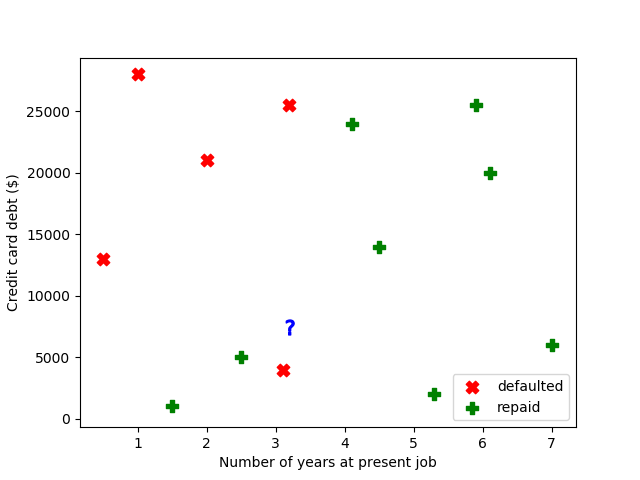
\includegraphics[width=0.9\textwidth]{bank_training.png}
\caption{Training data for a bank's home mortgage operations.}
\label{bank_training}
\end{figure}

\index{Mr.~Blue Question Mark}
Now suppose Mr.~Blue Question Mark walks in. Should we approve his loan
application? A 1-NN classifier would say \textit{no}, since the closest data
point to the blue question mark is a red X. A 3-NN classifier, on the other
hand, would say \textit{yes}, since if we take the three nearest neighbors of
the question mark, we get two greens and one red. (See
Figure~\ref{bank_training_13nn}.)

\begin{figure}[ht]
\centering
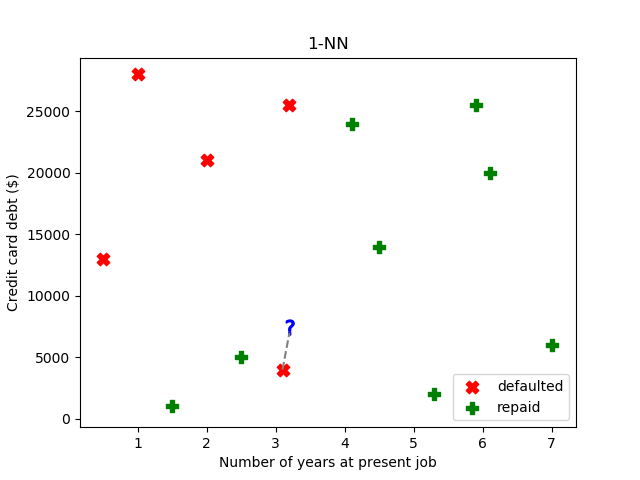
\includegraphics[width=0.48\textwidth]{bank_training_1nn.png} \ 
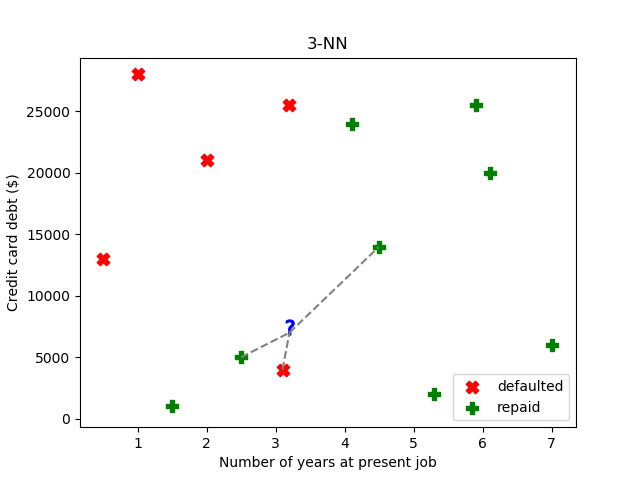
\includegraphics[width=0.48\textwidth]{bank_training_3nn.png}
\caption{The 1, and 3, ``closest'' points to our mystery man.}
\label{bank_training_13nn}
\end{figure}

\section{Distance measures}

\index{distance measure}
\index{Euclidean distance}
\index{Pythagorean Theorem}
\index{straight-line distance}
\index{crow-flies distance}

Much hinges on the question of \textit{closeness}. What do we mean when we say
two data points are ``close'' together? There are some options here, many of
which are common sense. The approach we used above was to take the ordinary
\textit{Euclidean distance}, also called the ``straight-line distance'' (or
``crow-flies distance'') between the data points. We just use the Pythagorean
Theorem where each feature is plotted on an axis. And in fact this is the most
common choice.

You probably remember the formula for the distance between two points in a
plane. Less well known is that the Pythagorean formula works \textit{in any
number of dimensions}. In other words, if I have one $n$-dimensional data point
whose values are $(x_1, x_2, x_3, ..., x_n)$ and another whose are $(y_1, y_2,
y_3, ..., y_n)$, the distance between them is:

\vspace{-.15in}
\begin{align*}
d = \sqrt{(x_1-y_1)^2 + (x_2-y_2)^2 + (x_3-y_3)^2 + \dots + (x_n-y_n)^2}
\end{align*}
\vspace{-.15in}

You can't visualize more than three dimensions (and most people can do only
two), but you can compute it, and you get a perfectly sensible number.

\index{distance measure}
\index{taxicab distance}
\index{Manhattan distance}
This isn't the only approach people use. In general, we can use any
\textbf{distance measure} (or ``distance function,'' or ``distance metric'')
that assigns a numerical ``distance'' value to any two points. To be valid, a
distance measure must simply satisfy certain common sense
rules.\footnote{Including: the distance between two points must always be
greater than or equal to 0; the distance from $x$ to $y$ must be the same as
the distance from $y$ to $x$; and the distance from $x$ to $z$ must not be any
greater than the distance from $x$ to $y$ to $z$ (the ``triangle
inequality.'')} Another common choice is the \textbf{Manhattan distance} (or
``taxicab distance'') which is essentially the shortest path between the two
points that doesn't travel diagonally (\textit{i.e.}, the path only travels
along axes.)

\section{Feature standardization}

Now I actually did something sneaky to you with the bank example. When I showed
you the plots, I calculated the crow-flies distances to Mr.~Blue Question Mark
\textit{as they appeared on the page}. But if you look at the scales of those
axes, you'll realize I didn't compute them right! These variables are on vastly
different scales. In terms of absolute differences, the amount of credit card
debt, measured in the tens of thousands, completely overwhelms the work
history, which is at most a few decades. Taking the straightforward Euclidean
distance between two people, then, would actually be quite a blunder: clearly a
difference of \$50 of credit card debt isn't nearly as significant as a
difference of 50 years in seniority!

To make this concrete, the underlying data for Figures~\ref{bank_training} and
\ref{bank_training_13nn} is here:

\begin{Verbatim}[fontsize=\small,samepage=true,frame=single,framesep=3mm]
print(bank)
\end{Verbatim}
\vspace{-.2in}

\begin{Verbatim}[fontsize=\small,samepage=true,frame=leftline,framesep=5mm,framerule=1mm]
                       num_yrs  cc_debt  default
                    0      1.0    28000      yes
                    1      0.5    13000      yes
                    2      1.5     1000       no
                    3      2.0    21000      yes
                    4      2.5     5000       no
                    5      3.1     4000      yes
                    6      3.2    25500      yes
                    7      4.1    24000       no
                    8      4.5    14000       no
                    9      5.3     2000       no
                    10     5.9    25500       no
                    11     6.1    20000       no
                    12     7.0     6000       no
                    13     3.2     7500    maybe
\end{Verbatim}

Let's compute the Euclidean distance from each of the points to Mr.~Blue
Question Mark (row \#13), and sort by that new column (remember that in Python, 
\texttt{**} is used for ``to-the-power-of''):

\index{sqrt@\texttt{sqrt()} (NumPy)}

\begin{Verbatim}[fontsize=\small,samepage=true,frame=single,framesep=3mm]
pts_dist = np.array([])
for row in bank.itertuples():
    pts_dist = np.append(pts_dist,
        np.sqrt((row.cc_debt - 7500)**2 + (row.num_yrs - 3.2)**2))
bank['dist'] = pts_dist
print(bank.sort_values('dist'))
\end{Verbatim}
\vspace{-.2in}

\begin{Verbatim}[fontsize=\small,samepage=true,frame=leftline,framesep=5mm,framerule=1mm]
                 num_yrs  cc_debt  default          dist
            13       3.2     7500    maybe      0.000000
            12       7.0     6000       no   1500.004813
            4        2.5     5000       no   2500.000098
            5        3.1     4000      yes   3500.000001
            9        5.3     2000       no   5500.000401
            1        0.5    13000      yes   5500.000663
            8        4.5    14000       no   6500.000130
            2        1.5     1000       no   6500.000222
            11       6.1    20000       no  12500.000336
            3        2.0    21000      yes  13500.000053
            7        4.1    24000       no  16500.000025
            6        3.2    25500      yes  18000.000000
            10       5.9    25500       no  18000.000202
            0        1.0    28000      yes  20500.000118
\end{Verbatim}

It's madness. The ``closest'' point to Mr.~Blue is the one with a
\texttt{num\_yrs} of 7 and a \texttt{cc\_debt} of 6000...the green point that's
pegged all the way to the right side of the plot! (See
Figure~\ref{bank_training}.)

If you think it through, you'll realize why. Moving left-or-right on this plot
is cheap; it's differences in \textit{vertical} position that generate large
distances. The far-right green plus really \textit{is} very close to Mr.~Blue,
because her credit card debt is very close to his (\$6,000 vs. \$7,500). Her 7
years of consecutive work history compared to his 3.2 just isn't a factor,
because it's measured in single digits.

\index{standardization}
\index{normalized (variable)}
\index{Z-score}

This is a very common issue with data sets, and fortunately, there's an easy
way around it. Instead of using the absolute numbers in our Pythagorean formula
calculation (or Manhattan distance calculation, or whatever), we first
\textbf{transform} our features so they are all \textbf{standardized} (or
``\textbf{Z-score normalized}\footnote{This definition of the term
``normalized'' has nothing to do with the normalization of data sets we learned
about in Sections~\ref{normalized} and \ref{normalized2}, btw.}.'') All we have
to do is take each feature, and:

\begin{compactenum}
\item subtract its mean from each point, then
\item divide each point by its standard deviation.
\end{compactenum}

This puts all features on the same level playing field, so to speak. If you
remember from your stats class, what we've done is compute the \textbf{Z-score}
for each data point: the number of standard deviations above (or below) the
mean it is. Now no feature gets an advantage in the distance calculation over
any other feature, even if they're on wildly different scales: 2.5 standard
deviations is 2.5 standard deviations, no matter what the underlying units.

Here's code to do that with the bank example:

\begin{Verbatim}[fontsize=\small,samepage=true,frame=single,framesep=3mm]
def zscores(arr):
    return (arr - arr.mean()) / arr.std()

bank.cc_debt = zscores(bank.cc_debt)
bank.num_yrs = zscores(bank.num_yrs)
\end{Verbatim}

Now, if we compute distances with these Z-scores, instead of the raw values, we
get something that looks much more reasonable:

\begin{Verbatim}[fontsize=\small,samepage=true,frame=single,framesep=3mm]
zscore_dist = np.array([])
for row in bank.itertuples():
    zscore_dist = np.append(zscore_dist,
        np.sqrt((row.cc_debt - bank.iloc[len(bank)-1].cc_debt)**2 +
            (row.num_yrs - bank.iloc[len(bank)-1].num_yrs)**2))
bank['dist'] = zscore_dist
print(bank.sort_values('dist'))
\end{Verbatim}
\vspace{-.2in}

\begin{Verbatim}[fontsize=\small,samepage=true,frame=leftline,framesep=5mm,framerule=1mm]
                 num_yrs    cc_debt  default      dist
            13 -0.181877  -0.667388    maybe  0.000000
            5  -0.231804  -1.024786      yes  0.360869
            4  -0.531366  -0.922673       no  0.432797
            8   0.467174  -0.003647       no  0.928342
            2  -1.030636  -1.331128       no  1.077471
            9   0.866590  -1.229014       no  1.189415
            1  -1.529906  -0.105761      yes  1.460345
            3  -0.781001   0.711151      yes  1.503103
            7   0.267466   1.017493       no  1.743769
            6  -0.181877   1.170664      yes  1.838051
            12  1.715350  -0.820559       no  1.903400
            11  1.266006   0.609037       no  1.930188
            10  1.166152   1.170664       no  2.279389
            0  -1.280271   1.425948      yes  2.364006
\end{Verbatim}

The data is plotted on Z-score normalized axes in
Figure~\ref{bank_training_zscore}. As you can see, the nearest neighbor to
Mr.~Blue is the point .023 standard deviations lower than the mean job
seniority, and 1.02 standard deviations lower than the mean credit card debt,
which is precisely the red X nearest to the question mark.

\begin{figure}[ht]
\centering
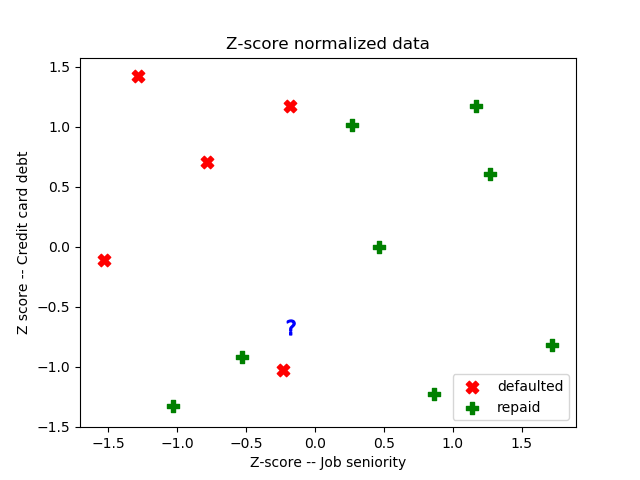
\includegraphics[width=0.9\textwidth]{bank_training_zscore.png}
\caption{Both variables have been Z-score normalized (note the axis scales)!}
\label{bank_training_zscore}
\end{figure}


\section{Categorical features}

Now what do we do if our features are categorical? We can just make them
numerical, but in a principled way. If we have a binary feature, with only two
possible values -- \texttt{public}/\texttt{private},
\texttt{collegeGraduate}/\texttt{notACollegeGraduate} -- it's easy: we just
assign one number (say, ``1'') to one value and another (``2'') to the other
one. Now we've turned a categorical column of
\texttt{employed}-or-\texttt{unemployed}'s into a numeric column of 1-or-2's,
which lets us compute Z-scores and distance measures as we did above.

\index{baseball}
\index{football}
\index{lacrosse}

With more than two possible values, though, you have to be careful. Consider a
feature whose three values are ``\texttt{baseball},'' ``\texttt{football},''
and ``\texttt{lacrosse}.'' Many people might unsuspectingly assign the numbers
1, 2, and 3 to these values and then treat the feature as a numeric one. But
you can't do this. Here's why: assuming the original values were on a
categorical/nominal scale (recall the ``Scales of Measure'' chapter from Volume
I of this series), converting them to numbers in a simpleminded fashion like
this \textit{imposes an interval scale where none exists.}

Think about it. A person whose favorite sport is baseball isn't any
\textit{more} like a football fan than she is like a lacrosse fan. Yet if we
turn \texttt{baseball} into 1, \texttt{football} into 2, and \texttt{lacrosse}
into 3, that's exactly what our kNN classifier is going to think. It will view
baseball fans and lacrosse fans as ``further apart'' because after all, 3 minus
1 is 2.

\index{one-hot encoding}

In order to avoid biasing the classifier with this non-information, we use a
technique called \textbf{one-hot encoding}. We turn each categorical feature
into a whole \textit{set} of binary features, one for each value. So instead of
a \texttt{sport} feature with values \texttt{baseball}, \texttt{football}, and
\texttt{lacrosse}, we use \textit{three} features -- called \texttt{baseball},
\texttt{football}, and \texttt{lacrosse} -- each with values of 0 or 1.
Example:

\begin{center}
\footnotesize
\begin{tabular}{|c|c|c|}
\hline
age & edLevel & sport \\
\hline
37 & HS & football \\
41 & college & baseball \\
19 & college & football \\
22 & college & lacrosse \\
\hline
\end{tabular}
\quad
{\Huge $\Rightarrow$}
\quad
\begin{tabular}{|c|c|c|c|c|c|}
\hline
age & HS & college & football & baseball & lacrosse \\
\hline
37 & 1 & 0 & 1 & 0 & 0 \\
41 & 0 & 1 & 0 & 1 & 0 \\
19 & 0 & 1 & 1 & 0 & 0 \\
22 & 0 & 1 & 0 & 0 & 1 \\
\hline
\end{tabular}
\end{center}

\index{wide form}
\index{long form}

Perhaps you can see why it's called ``one-hot'' encoding: each row has exactly
one ``hot'' (\textit{i.e.}, 1) entry for each of the one-hotted features.
Specifically, every row has either a 0 for \texttt{HS} and a 1 for
\texttt{college}, or vice versa; and every row has a 1 for exactly \textit{one}
of \texttt{football}, \texttt{baseball}, and \texttt{lacrosse}, and 0 for the
other two. This is sort of like going from \textbf{long form} to \textbf{wide
form} data, if you think about it.

\index{scikit-learn@\texttt{scikit-learn} (package)}
\index{OneHotEncoder@\texttt{OneHotEncoder.fit\_transform()}}
\index{fit\_transform@\texttt{fit\_transform()}}
\index{sparse@\texttt{sparse=False} (\texttt{OneHotEncoder})}

You can use \texttt{np.where()} function to create one-hot features, or you
might find the \texttt{scikit-learn} package's
\texttt{OneHotEncoder.fit\_transform()} function helpful. It's a little weird;
when you create your \texttt{OneHotEncoder}, you have to pass it an argument of
``\texttt{sparse=False}'' if you want it to work the way you expect.

\index{import@\texttt{import}}
\index{double boxies@``double boxies''}
\index{[]@\texttt{[]} (boxies)}

\begin{Verbatim}[fontsize=\small,samepage=true,frame=single,framesep=3mm]
from sklearn.preprocessing import OneHotEncoder

ohe = OneHotEncoder(sparse=False)
onehot_features = ohe.fit_transform(df[['edLevel','sport']])
\end{Verbatim}

Careful: although this function takes a \texttt{DataFrame} as input, it returns
a \texttt{NumPy} array as output:

\begin{Verbatim}[fontsize=\small,samepage=true,frame=single,framesep=3mm]
print(df[['edLevel','sport']])
\end{Verbatim}
\vspace{-.3in}

\begin{Verbatim}[fontsize=\small,samepage=true,frame=leftline,framesep=5mm,framerule=1mm]
   edLevel     sport
0       HS  football
1  college  baseball
2  college  football
3  college  lacrosse
3    lacrosse
Name: sport, dtype: object
\end{Verbatim}

\begin{Verbatim}[fontsize=\small,samepage=true,frame=single,framesep=3mm]
print(onehot_features)
\end{Verbatim}
\vspace{-.3in}

\begin{Verbatim}[fontsize=\small,samepage=true,frame=leftline,framesep=5mm,framerule=1mm]
[[1. 0. 0. 1. 0.]
 [0. 1. 1. 0. 0.]
 [0. 1. 0. 1. 0.]
 [0. 1. 0. 0. 1.]]
\end{Verbatim}

\medskip
If you want these columns back in your \texttt{DataFrame}, you'll have to stick
them back in there:

\begin{Verbatim}[fontsize=\small,samepage=true,frame=single,framesep=3mm]
df['HS'] = onehot_features[:,0]
df['college'] = onehot_features[:,1]
df['baseball'] = onehot_features[:,2]
df['football'] = onehot_features[:,3]
df['lacrosse'] = onehot_features[:,4]
df = df.drop(['edLevel','sport'],axis=1)

print(df)
\end{Verbatim}
\vspace{-.3in}

\begin{Verbatim}[fontsize=\small,samepage=true,frame=leftline,framesep=5mm,framerule=1mm]
   age   HS  college  baseball  football  lacrosse
0   37  1.0      0.0       0.0       1.0       0.0
1   41  0.0      1.0       1.0       0.0       0.0
2   19  0.0      1.0       0.0       1.0       0.0
3   22  0.0      1.0       0.0       0.0       1.0
\end{Verbatim}

But as we'll see in the next chapter, the array itself is ready-made for
\texttt{scikit-learn}'s powerful classifier implementations. Stay tuned.
